\subsection{Prover Network}
In prover network, we are going to deploy a Jolt zkVM~\cite{jolt} based system. The Jolt zkVM is a cutting-edge zero-knowledge virtual machine designed for generating and verifying cryptographic proofs of program execution efficiently. It enables tamperproof computation, where the correctness of state transitions can be verified without revealing the underlying data. The Jolt zkVM is optimized for scalability, speed, and interoperability, making it well suited for handling complex blockchain operations and cross-chain transactions in a secure and trustless manner.  

Key Features of Jolt zkVM: 
\begin{itemize}
    \item \textsf{High Performance}: Leverages advanced proof systems to reduce proving and verification times, ensuring rapid state transitions.  
    \item \textsf{Flexibility}: Supports a modular design, allowing different modules (e.g., EVM, SVM, WASM, MoveVM) to operate in isolation while sharing a common infrastructure.  
    \item \textsf{Scalability}: Designed to handle large-scale computations by supporting distributed execution, enabling parallelized proof generation.  
    \item \textsf{Interoperability}: Compatible with various blockchain environments, making it ideal for cross-chain solutions.  
\end{itemize}


The Jolt zkVM combines high performance with modularity, enabling it to outperform competitors in handling cross-chain operations and isolated state management. Unlike others, it supports a truly modular design in which multiple VM modules can coexist, maintaining isolated states for different blockchains.  

\begin{figure}[h]
    \centering
    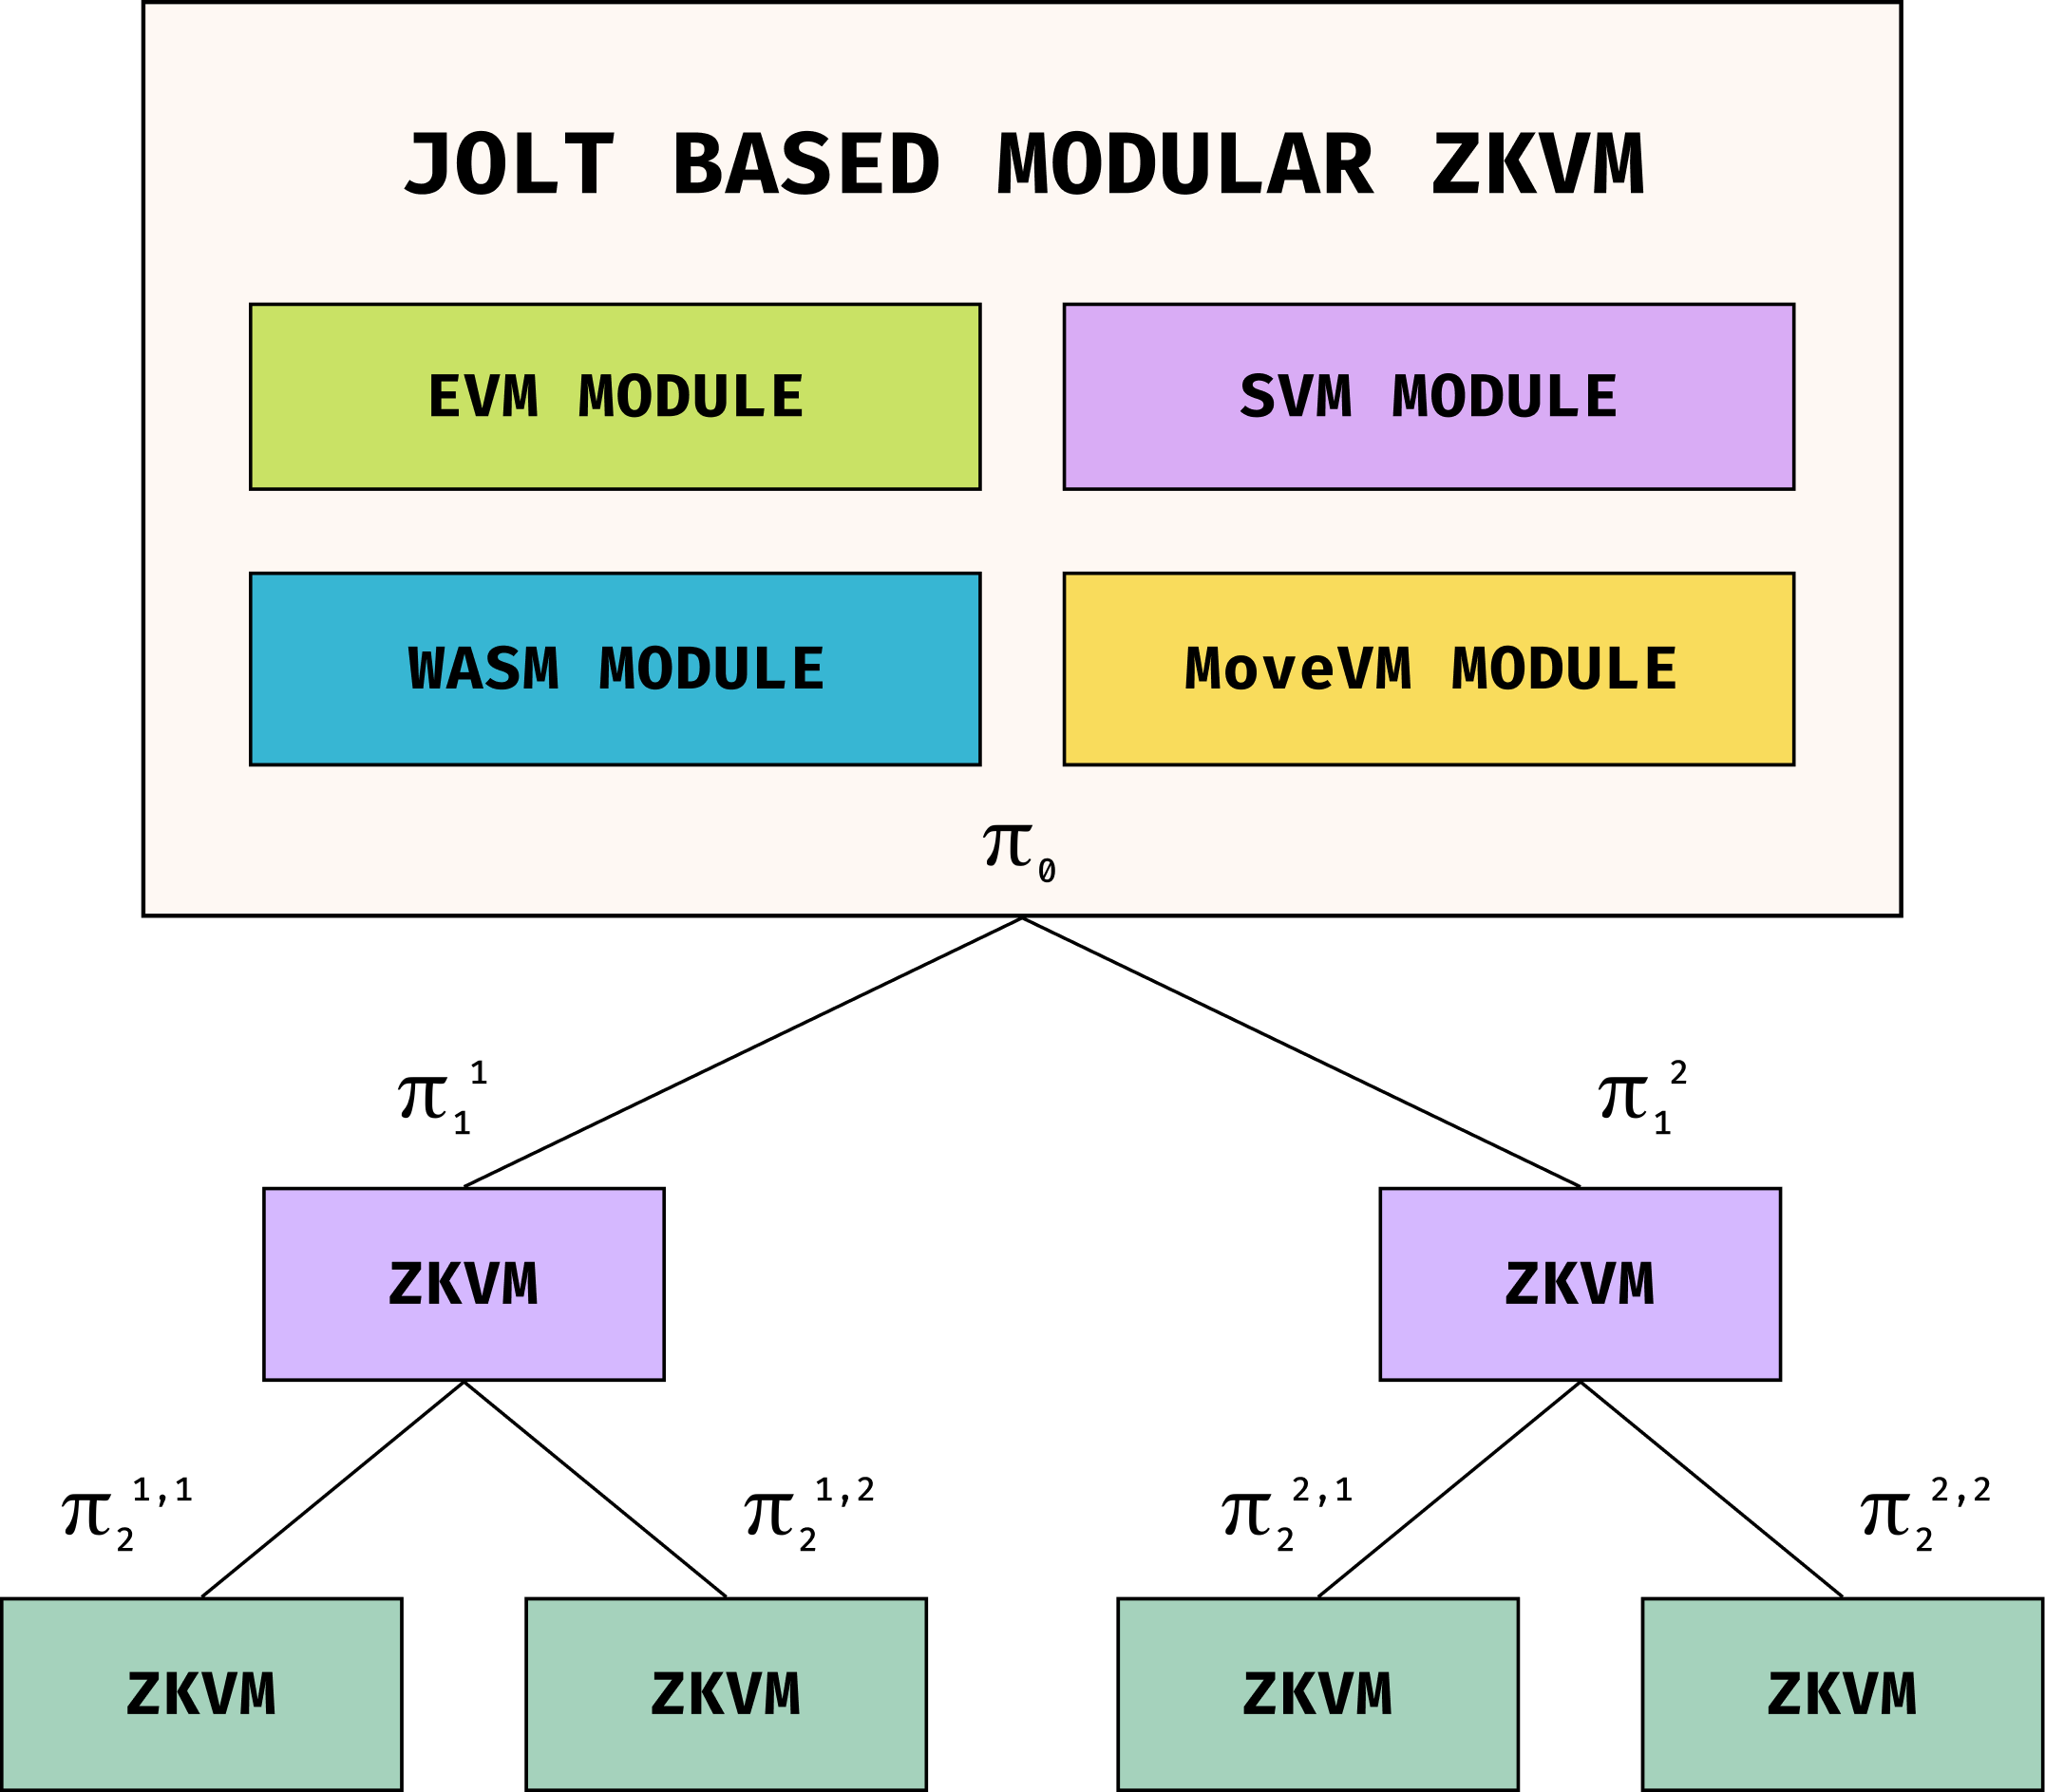
\includegraphics[width=0.7\linewidth]{figure/prover.png}
    \caption{Prover Network}
    \label{fig:prover}
\end{figure}

\subsubsection{Jolt zkVM}
The paper~\cite{jolt} introduces a novel approach to building zero-knowledge virtual machines (zkVMs) by leveraging a technique called Jolt. This method focuses on transforming program execution into a series of lookups into a predetermined, extensive lookup table, thereby enhancing efficiency and auditability in zkVMs. 

\begin{itemize}
    \item Lookup Singularity Vision: Jolt realizes the "lookup singularity" concept, aiming to design circuits that primarily perform lookups into a massive, predetermined table. This table, dependent solely on the instruction set architecture (ISA), is structured to avoid costs that scale linearly with its size, despite its theoretical enormity (e.g., size exceeding $2^128$). 

    \item Lasso Lookup Argument: To validate the lookups efficiently, Jolt employs a new lookup argument called Lasso, detailed in a companion work by Setty, Thaler, and Wahby. Lasso enables efficient proofs of correct execution by performing multiple lookups into smaller subtables and combining the results, facilitating the handling of massive structured tables without incurring prohibitive costs. 

    \item Application to RISC-V ISA: The paper demonstrates the application of Jolt to the RISC-V ISA, a widely adopted open standard. For 64-bit data types, the dominant cost for the Jolt prover is cryptographically committing to approximately six 256-bit field elements per RISC-V CPU step. This performance is favorable compared to prior zkVM providers, even those focused on simpler VMs. 

    \item Performance and Auditability Benefits: Jolt offers significant performance improvements and enhanced auditability over previous zkVMs. By reducing complex computations to structured table lookups, it simplifies the verification process and reduces the computational burden on the prover, leading to more efficient and transparent zkVM implementations. 

\end{itemize}


\subsubsection{Distributed Deployment of Jolt zkVM}  

Deploying the Jolt zkVM in a distributed form brings several advantages by leveraging a network of provers to parallelize computation and enhance scalability.  Distributes computation of zk proofs across multiple nodes, significantly reducing the time required for proof generation.  Increases resilience by ensuring that proof generation can continue even if some nodes in the network fail. Dynamically allocates workloads across nodes, ensuring efficient resource utilization. By deploying nodes geographically closer to the data sources or target blockchains, latency is minimized, and overall throughput is enhanced.  

The modular architecture of the Jolt zkVM is the cornerstone of efficient and isolated state management across multiple blockchains. By integrating specialized virtual machine modules, such as the EVM Module, SVM Module, MoveVM Module, and WASM Module, the zkVM can simultaneously maintain the states of various chains in a unified, yet independent manner, ensuring both interoperability and operational isolation. The EVM Module is designed to handle Ethereum-compatible chains, providing robust support for Solidity-based smart contracts and facilitating seamless state transitions within the Ethereum ecosystem. The SVM Module caters to Solana-compatible chains, leveraging Solana's high-performance architecture to enable rapid transaction processing and execution. The MoveVM Module enables compatibility with Move-based blockchains, such as Aptos and Sui, by using Move's resource-oriented programming model to enhance security, parallel execution, and asset integrity. The WASM Module supports chains based on WebAssembly (WASM), offering developers the flexibility to build and run applications in diverse programming languages such as Rust, C++, and more. 


This modularity not only enhances the zkVM's ability to manage cross-chain interactions efficiently but also provides a scalable framework for supporting an expanding ecosystem of blockchains with varying technical requirements. The combination of distributed deployment and modularity in the Jolt zkVM sets a new standard for zkVMs, providing unparalleled scalability, flexibility, and cross-chain capabilities to power the next generation of blockchain applications.